\documentclass{article} %this is an article
\usepackage[lmargin=.75in,rmargin=.75in,tmargin=1.in,bmargin=1in]{geometry} % setting margins
%\usepackage{tree-dvips}
\usepackage{tikz}  %makes crazy graphs
\usepackage{enumitem}
% \usetikzlibrary{snakes}
%\usepackage[flushleft]{threeparttable} %% makes notes for tables that wraps around width of table
%\usepackage{chronology}
\usepackage[round]{natbib}  %% beatiful bibliography
%\usepackage{wrapfig}
%\usepackage{longtable} %%multipage table
%\usepackage{qtree}
\usepackage{verbatim} %all kinds of shit
\usepackage{graphicx} %beautiful figures
%\usepackage{graphics}
%\usepackage{color}
%\usepackage{caption}
\usepackage{subcaption} %subcaption on the the subfigures
%\usepackage{multirow}
%\usepackage{sidecap}
%\usepackage{epstopdf}
\usepackage{amssymb} %beautiful math
\usepackage{amsmath,amssymb,amsfonts,amsthm,array} %beautiful math
\usepackage{amsthm}  %beautiful math
\usepackage{pgfplots}  %Normal distribution figure
\usepackage[colorlinks=true,linkcolor=red, citecolor=red]{hyperref} %sets my preferences for cross reference



\begin{document}
\section{Lucas \& Stokey 1983}
The model features
\begin{itemize}
  \item a government that must finance an exogenous stream of
    government expenditures with either
    \begin{itemize}
     \item  flat rate tax on labor, or
     \item purchases and sales from a full array of Arrow
        state-contingent securities
    \end{itemize}
  \item a representative household that values consumption and leisure
    \item a linear production function mapping labor into a single
      good
    \item a Ramsey planner who at time $t=0$ chooses a plan for
        taxes and trades of Arrow securities for all $t \geq 0$
 \end{itemize}
%%%%%%%%%%%%%%%%%%%%%%%%%%%%%%%%%%%%%%%%%%%%%%%%%%%%%%%%%%%%%%%%%
 \subsection{The model}
 For $t \geq 0$, history $s^t = [s_t,s_{t-1},...,s_0]$ of an exogenous
 state $s_t$ has joint probability density $\pi(s_t)$. Government
 purchases $g_t(s^t)$ at time $t \geq 0$ depend on $s^t$. Let
 $c_t(s^t),l_t(s^t)$, and $n_t(s^t)$ denote consumption, leisure, and
 labor supply. The representative household is endowed with one unit of time that can be divided between leisure $l_t$ and labor $n_t$ such that 
%
\begin{equation}
  n_t(s^t) + l_t(s^t) = 1 \label{eqn:time}
\end{equation}
%
Household preferences are of infinite horizon over consumption and
leisure and satisfy the usual conditions
%
\begin{equation}
\sum_{t=0}^{\infty} \sum_{s^t} \beta^t \pi(s^t) u(c_t(s^t),l_t(s^t)) \label{eqn:preferences}
\end{equation}
%
output equals $n_t(s^t)$ and can be divided between consumption and government purchases. Below are the equations that will be used to define the problem:
%
\begin{equation}
 c_t(s^t) + g_t(s^t) = n_t(s^t) \label{eqn:feasibility}
\end{equation}
%
\begin{equation}
g_t(s^t) = \tau_t(s^t)n_t(s^t) + \sum_{s^{t+1}} p_{t+1}(s_{t+1}|s^t) b_{t+1}(s_{t+1}|s^t) - b_{t}(s_{t}|s^{t-1}) \label{eqn:GB}
\end{equation}
%
\begin{equation}
c_t(s^t) + \sum_{s^{t+1}} p_t(s_{t+1}|s^t) b_{t+1}(s_{t+1}|s^t)  = [1 -\tau_t(s^t)]n_t(s^t) + b_{t}(s_{t}|s^{t-1}) \;\; \forall t\geq 0 \label{eqn:HB}
\end{equation}
%
Now we'll define allocations in the economy:
%
\begin{itemize}
\item government policy is $\{g(s^t) \}_{t=0}^{\infty}, \{\tau(s^t) \}_{t=0}^{\infty}$
\item feasible allocation is a consumption labor supply plan $\{c(s^t),n(s^t) \}_{t=0}^{\infty}$
\item price system is a sequence of Arrow security prices $\{p_{t+1}(s_{t+1}|s^t)\}_{t=0}^{\infty}$
\end{itemize}
%
Arrow Debreu prices can be defined as:
%
$$q_{t+1}^0(s^{t+1}) = p_{t+1}(s_{t+1}|s^t) q_{t}^0(s^{t})$$
%
And by exploring the recursion of the household budget constraint and
plugging in A-D prices, we get the following present-value budget
constraint:
%
\begin{equation}
\sum_{t=0}^{\infty} \sum_{s^t} q_{t}^0(s^{t}) c_t(s^t) = \sum_{t=0}^{\infty} \sum_{s^t} q_{t}^0 [1 - \tau_t(s^t)]n(s^{t}) +  b_0 \label{eqn:present_value_BC}
\end{equation}
%
Household problem is to choose $\{c(s^t),n(s^t) \}_{t=0}^{\infty}$  to
maximize \ref{eqn:preferences} wrt constraints \ref{eqn:time} and \ref{eqn:HB} for all $t,s^t$ whose FOC is:
%
\begin{equation}
(1 - \tau_t(s^t)) = \frac{u_l(s^t)}{u_c(s^t)} \label{eqn:mris}
\end{equation}
%
\begin{equation}
p_{t+1}(s_{t+1}|s^t) = \beta^t \pi_t(s_{t+1}|s^t) \frac{u_c(s^{t+1})}{u_c(s^t)}  \Rightarrow 
\;\;q_{t}^0(s^t) = \beta^t \pi_t(s^t) \frac{u_c(s^{t})}{u_c(s^0)} \label{eqn:ee}
\end{equation}
%
Finally, using equations \ref{eqn:mris} and \ref{eqn:ee} to eliminate taxes and prices from \ref{eqn:present_value_BC}, we derive the implementability constraint:
%
\begin{equation}
\sum_{t=0}^{\infty} \sum_{s^t} \beta^t \pi_t(s^t)[u_c(s^t)c_t(s^t) - u_l(s^t)n_t(s^t)]  - u_c(s^0)b_0 = 0 \label{eqn:ic}
\end{equation}
% 
%
\subsection{Solving the model}
The Ramsey problem is to maximize \ref{eqn:preferences}  constrained
by equation \ref{eqn:ic}, ie, the single implementatbility constraint and feasibility. We can write the problem
\\
at $t \geq 1$
%%
\begin{align}
V(x,s) = & \max_{c(s),n(s),x'(s')} u(c(s),1-n(s)) + \beta \sum_{s'} \Pi(s'|s) V(x',s') \nonumber \\
  s.t.\;    & x = u_c(s)c(s) - u_n(s)n(s) + \beta \sum_{s' \in S} \Pi(s'|s)x'(s')  \nonumber \\
  & n(s) = c(s) + g(s) \nonumber
\end{align}
%%
And at $t=0$
\begin{align}
V(b_0,s_0) = & \max_{c_0,n_0,x'(s_1)} u(c_0,1-n_0) + \beta \sum_{s_1} \Pi(s_1|s_0) V(x'(s_1),s_1) \nonumber \\
  s.t.\;    & x = u_{c,0}(c_0) - u_{n,0}n_0 + \beta \sum_{s_1 \in S} \Pi(s_1|s_0)x'(s_1) \nonumber \\
  & n_0 = c_0 + g_0 \nonumber
\end{align}
%%
%%
%In
%order to solve this problem, first write the pseudo utility:
%$$V[c_t(s^t),n_t(s^t),\phi] = u(c_t(s^t),1 - n_t(s^t))  + \phi[u_c(s^t) c_t(s^t) - u_l(s^t) n_t(s^t)]$$
%
%Next define the following Lagrangean:
%
%$$ \sum_{t=0}^{\infty} \sum_{s^t} \beta^t \pi(s^t) \left\{ V[c_t(s^t),n_t(s^t),\phi] + \theta_t(s^t)[n_t(s^t) - c_t(s^t) - g_t(s^t)]\right\} - \phi u_c(0) b_0 $$
%
%where $\{\theta_t(s^t)\}_{t=0}^{\infty}$ is a sequence of langrange multipliers on the feasibility conditions. We can then obtain the FOCs of the Ramsey problem as follows:
%%
Then we can take first order conditions to get $t \geq 1$
\begin{align}
&c_t(s^t): \;\; (1+ \phi)u_c(s^t) + \phi[u_{cc}(s^t)c_t(s^t) - u_{lc}(s^t)n_t(s^t)] - \theta_t(s^t) = 0  \\
&n_t(s^t): \;\; -(1+ \phi)u_l(s^t) - \phi[u_{cl}(s^t)c_t(s^t) - u_{ll}(s^t)n_t(s^t)] + \theta_t(s^t) = 0 
\end{align}
for $t = 0$
\begin{align}
&c_0(s^0,b_0): \;\; (1+ \phi)u_c(s^0,b_0) + \phi[u_{cc}(s^0,b_0)c_0(s^0,b_0) - u_{lc}(s^0,b_0)n_0(s^0,b_0)] - \theta_0(s^0,b_0) - \phi u_{cc}(s^0,b_0)b_0 = 0 \\
&n_0(s^0,b_0): \;\; -(1+ \phi)u_l(s^0,b_0) + \phi[u_{cl}(s^0,b_0)c_0(s^0,b_0) - u_{ll}(s^0,b_0)n_0(s^0,b_0)] + \theta_0(s^0,b_0) + \phi u_{cl}(s^0,b_0)b_0 = 0 
\end{align}
In SL, we have one implementability constraints and a time 1 problem for any given $\phi$ and then we back out $\phi$ based on the time 0 problem. To solve the time 1 problem we use the first best allocation. As seen above, the time 1 problem is independent of debt and only depend on the realization of $g$, however, the time 0 problem depends on both $g_0$ and $b_0$.
%%
\\
\\
We need another equation to determine $\phi$. Note that the time inconsistency in this problem comes from the fact that debt affects the time 0 decision but does not affect the decision onwards. This reenforces the idea that if given the opportunity to change the policy at any point in time, the gov't is subject to a different $b_0$ and would choose to change their position. Now , as for $\phi$, it has to take a value that assures that the government's budget constraints are both satisfied at a candidate Ramsey allocation and price system associated with that $\phi$ 
%%
\\
\\
Note that substituting  \ref{eqn:mris}, \ref{eqn:ee} and  \ref{eqn:feasibility} into the recursive form of the the HHD budget - equation  \ref{eqn:HB} - we get:
%%
$$u_c(s^t)[n_t(s^t) - g_t(s^t)] + \beta \sum_{s_{t+1}} \pi(s_{t+1}|s_t) u_c(s^{t+1})b_{t+1}(s_{t+1}|s^t)  = 
u_l(s^t)n_t(s^t) + u_c(s^t)b_t(s_t|s^{t-1})$$
%%
We can then define an alternative state variable $x_t(s^t) = u_c(s^t)b_t(s_t|s^{t-1})$ and the equation can be rewritten as:
%%
$$u_c(s)[n_t(s) - g_t(s)] + \beta \sum_{s'} \pi(s'|s) x'(s')  = u(s)n(s) + x(s)$$
%%
And in matrix form we have:
%%
$$ \vec{u}_c(\vec{n} - \vec{g}) + \beta \Pi \vec{x} = \vec{u}_l \vec{n} + \vec{x} \Rightarrow 
\vec{x} = (I - \beta \Pi)^{-1}[\vec{u}_c(\vec{n} - \vec{g}) - \vec{u}_l \vec{n}] $$
%%
Once we have $\vec{x}$, we can find $\vec{b}$ from $b(s) = \frac{x(s)}{u_c(s)}$ (i.e. element by element division)
%%
Hence we'll solve the model for a range of initial debt within a grid that is defined by the minimum of the first best debt allocation and its negative as the maximum. We guess values for $n_0,n(0.1),n(0.2)$, and $\phi$ which all come from the first best allocation as well (with a guess for $\phi = 0$) and a guess for every $b$ after $b_{min}$ as the allocation solved for the previous $b$
%%
\subsection{Computation}
Taking first order conditions of the continuation problem delineated above, we need to solve for $(c(s),l(s),\xi(s),x(s)$
\begin{align}
& u_c(s) + \phi[u_{cc}(s)c(s) + u_c(s)] - \xi(s) = 0 \;\; s\in S \\
& u_l(s) - \phi[u_{ll}(s)n(s) + u_l(s)] + \xi(s) = 0 \;\; s\in S \\ 
& l(s) - c(s) - g(s) \;\; s\in S
\end{align}
Use a nonlinear root solver to find $c(s),l(s)$, and $\theta(s)$ that solves the system above, then use the equation below:
%%
$$\vec{x} = (I - \beta \Pi)^{-1}[\vec{u}_c(\vec{n} - \vec{g}) - \vec{u}_l \vec{n}]$$
%%
to solve for $x(s)$. Solving the time 0 problem entails using the $x(s)$ solved in the continuation problem and using a nonlinear root solver to solve for $(c(s_0),l(s_0),\xi_0(s_0),\mu)$ on the following system:
\begin{align}
&u_{c0}b_0 = u_{c0}(n_0 - g_0) - u_{l0} n_0 + \beta \sum_{s=1}^S\pi(s|s0)x(s) \\
& u_{c}(s_0) + \phi[u_{cc}(s_0)c_t(s_0) + u_c(s_0)] - \xi_0(s_0) = 0  \\
& u_l(s_0) - \phi[u_{ll}(s_0)n(s_0) + u_l(s_0)] + \xi(s_0) = 0 \\ 
& l(s_0) - c(s_0) - g(s_0)
\end{align}
%%%%
\section{Aiyagari, Marcet, Sargent \& Seppala 2002}
The problem is now posed differently. Instead of having only one implementability constraint, there are as many implementability constraint as the number of states. The incompleteness here comes from not being about to buy state contingent debt. The problem can be posed recursively as follows. Preferences follow:
\begin{equation}
  U(c,l) = \frac{c^{1-\alpha} - 1}{1-\alpha} - \frac{l^{1+\gamma}}{1+\gamma} \label{eqn2:preferences}
\end{equation}
%%%
As in SL, use the MRIS and EE in order to eliminate taxes from the budget constraint and arrive at the implementability constraints below:
%%
\begin{equation}
u_c(s)c_t(s^t) - u_l(s^t)n_t(s^t)]  + x(s) = \frac{x\_ p(s)}{\beta E_s[p(s)u_c(s)]} \label{eqn2:ic}
\end{equation}
%%
Then, the problems at time 0 and 1 can be written as follows
\begin{align}
V(x\_) = & \max_{c(s),n(s),x'(s')} \sum_{s} \Pi(s) u(c(s),l(s)) + \beta V(x(s)  \nonumber \\
  s.t.\;    & x(s) + u_c(s)c(s) - u_l(s)l(s) = \frac{x\_ p(s)}{\beta E_s[p(s)u_c(s)]} \;\; \forall s \in S    \label{amss_IC} \\
  & n(s) = c(s) + g(s) \;\; \forall s \in S \label{amss_feasibility}
\end{align}
%%
And at $t=0$
\begin{align}
V(b_0) = & \max_{c_0,l_0}  u(c_0,l_0) + \beta  V(u_c(s_0)b_0,s_0) \nonumber \\
  s.t.\;    & b_0 + u_{c,0}c_0  - u_{n,0}n_0 = \frac{b_0p(s_0)}{\beta} \nonumber \\
  & n_0 = c_0 + g_0 \nonumber
\end{align}
Taking FOC's and writing them recursively in $\mu$, we have:
\begin{align}
  c(s): & \;\; u_c(c_{s,s\_}(\mu)) - \mu'_{s,s\_}(\mu)[u_{cc}(c_{s,s\_}(\mu))c_{s,s\_}(\mu) + u_c(c_{s,s\_}(\mu))] - \nonumber \\ & \frac{u_{cc}(c_{s,s\_}(\mu))x_{s\_}(\mu) p(s)}{\beta E_{s\_}[p u_c(c(\mu))]}(\mu'_{s,s\_}(\mu) - \mu) - \xi_{s,s\_}(\mu) \;\; \forall s \in S    \label{amss_foc_c} \\
   l(s): & \;\; u_l(l_{s,s\_}(\mu)) - \mu'_{s,s\_}(\mu)[u_{ll}(l_{s,s\_}(\mu))l(s) + u_l(l_{s,s\_}(\mu))] +  \xi_{s,s\_}(\mu) \;\; \forall s \in S    \label{amss_foc_l} \\
   x(s): & \;\; E_{s\_}\mu'_{s,s\_}(\mu)\left[\frac{u_c(c_{s,s\_}(\mu))p(s)}{E_{s\_}u_c(c(\mu))p}\right] =  \mu\_     \label{amss_foc_x}
\end{align}
\subsection{Computation}
Equations \ref{amss_IC} (s equations), \ref{amss_feasibility} (s equations), \ref{amss_foc_c}(s equations), \ref{amss_foc_l} (s equations), and \ref{amss_foc_x} (1 equation) make up the system of $4s+1$ equations. We'll use the lagrange multiplier as a state variables. Then define a grid on $\mu$. Write this system as $F(x\_,\xi_{s\_,s}(\mu\_),l_{s\_,s}(\mu\_),\xi_{s\_,s}(\mu\_),\xi_{s\_,s}(\mu\_),\mu'_{s\_,s}(\mu\_)|\mu\_,s\_)=0$. Writing the system recursively in $\mu$ requires us to rewrite the two original constraints also as functions of $\mu$ as follows:
\begin{align}
& x_s(\mu'_{s\_,s}(\mu)) + u_c(c_{s,s\_}(\mu))c_{s,s\_}(\mu) - u_l(l_{s,s\_}(\mu))l_{s,s\_}(\mu) = \frac{x_{s\_}(\mu) p(s)}{\beta E_s[pu_c(c(\mu))]} \;\; \forall s \in S    \label{amss_IC} \\
  & l_{s,s\_}(\mu) = c(s)c_{s,s\_}(\mu) + g(s) \;\; \forall s \in S \label{amss_feasibility}
\end{align}

\begin{enumerate}
\item For each pair $(s\_,\mu\_)$, $\mu\_ \in [\mu_{min},\mu_{max}], s\_ \in S$
\item Guess $\left\{x_{s\_}^j(\mu\_) \right\}$ and use it as $x\_$ for $s\_$ and as an interpolating object to evaluate $x'(\mu'_{s,s\_}(\mu))$
\item Use $F(x_{s\_}(\mu\_),\xi_{s\_,s}(\mu\_),l_{s\_,s}(\mu\_),\xi_{s\_,s}(\mu\_),\xi_{s\_,s}(\mu\_),\mu'_{s\_,s}(\mu\_)|\mu\_,s\_)=0$ to solve for endogenous variables
\item Use $x_{s\_}(\mu\_)$ found in previous step to update the interpolating object to $\left\{x_{s\_}^{j+1}(\mu\_) \right\}$
\end{enumerate}
%%
\section{Simulations}
The AMSS model described above is precisely what was asked in lecture, i.e. the version of BEGS with only two states of government expenditure (high and low) and no uncertainty on P or $\Theta$. \\
\\
In this section I will simulate time series starting from an initial multiplier and state $(\mu_0, s_0)$. So although I solved the time-0 problem for LS, I did not do so for AMSS. I tested my soltution against the one in quantecon and got time series that resembed theirs. In fact, for the case in which utility is linear in consumption and strictly concave in leisure, I get that the series for taxes resemble a random walk. The case in which utility is concave on the other hand settles around a constant mean after a long period. Shown below are both the plots of various aggregates for both cases. Below is the intuition behind the two models. 

\subsection{Case 1: Preferences that are linear in consumption but concave in leisure}
When utility is linear in consumption and concave in leisure we get the result that taxes follow a random walk within some limit associated with the bounds on debt. As argued in the paper, this specification comes as close as possble to fullfilling Barro's result that taxes should be a random walk. As can see below with initial values $(\mu_0, s_0)= (-0.1,1)$. But

\begin{figure}
  \centering
  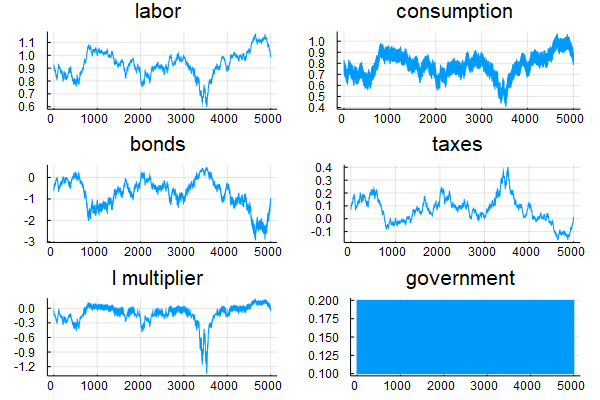
\includegraphics[width = 0.8\textwidth]{../debt_timeseries_linear.png}
    \caption{Preferences linear in consumption}
\end{figure}

\subsection{Case 2: Preferences that are concave in both consumption and leisure}
In this case, taxes at least in expected value converges to a near zero value. Consumption is much consistently higher after some time as can be seen below. In fact, this tells us that concavity of preferences in utility takes away the random walk trait of taxes as hypothesized by Barro. Further, we can see that getting Barro's result require stringent assumptions on utility. 

\begin{figure}
  \centering
  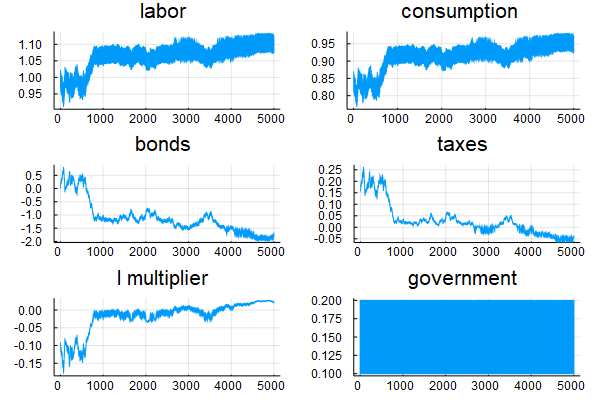
\includegraphics[width = 0.8\textwidth]{../debt_timeseries_concave.png}
    \caption{Preferences linear in consumption}
\end{figure}
% \bibliographystyle{plainnat}
%\bibliography{hw1.bib}
\end{document}
